\documentclass[a4paper]{article}
\usepackage[UTF8]{ctex}
\usepackage{tikz}
\usepackage{xcolor}
\usepackage{amsmath}
\usepackage{amsthm}
\usepackage{amssymb}
\usepackage{enumerate}
\usepackage{float}
\usepackage{arydshln}
\usepackage{listingsutf8}
\usepackage{listings-ext}
\usepackage[margin=1in]{geometry}
% https://www.latexstudio.net/archives/9774.html
% https://www.latexstudio.net/archives/2234
% https://texample.net/

\lstset{
    basicstyle=\tt,
    keywordstyle=\color{purple}\bfseries,
    identifierstyle=\color{brown!80!black},
    commentstyle=\color{gray}
    showstringspaces=false,
    breaklines=true % 自动换行
}

\newtheorem{theorem}{\indent 定理}[section]
\newtheorem{lemma}[theorem]{\indent 引理}
\newtheorem{proposition}[theorem]{\indent 命题}
\newtheorem{corollary}[theorem]{\indent 推论}
\newtheorem{definition}{\indent 定义}[section]
\newtheorem{example}{\indent 例}[section]
\newtheorem{remark}{\indent 注}[section]
\newenvironment{solution}{\begin{proof}[\indent\bf 解]}{\end{proof}}
\renewcommand{\proofname}{\indent\bf 证明}

\tikzset{eaxis/.style={->,>=stealth}}

\title{组合优化与凸优化作业2}

\author{HOMODELUNA}
\date{2025 年 4 月 13 日}

\begin{document}
\maketitle
\section{}

写代码,用共轭梯度法求解: \(\min f(x) = x_1 = x_2 + 2x_1^2 + 1x_1x_2 + x_2^2\)
,假设初始点 $x_0 = (0,0)^T, \epsilon = 10^{-6}$.

见: 

\section{}

写代码,用黄金分割法,斐波那契亚数列法,二分法,Shubert-Piyavskii分别求解问题:

\begin{enumerate}[(a)]
    \item \(min f(x) = 2x_2 -x -1\), 初始区间\( [a_0,b_0] = [-1,1]\),区间精度 \(\delta = 0.06\)
    
    \item \(\min f(x)=3x_2 - 21.6x-1\), 初始区间\([a_0,b_0] = [0,25]\),区间精度\(\delta = 0.08\)
    \item 
\end{enumerate}

见:

输出为:
\begin{lstlisting}
golden_section(test_1, -1, 1, 0.06) = Solution(0.25735421375199785, -1.1248918310801799)
golden_section(test_2, 0, 25, 0.08) = Solution(3.608630593568614, -39.879776538563966)
fibonacci_subsequence(test_1, -1, 1, 0.06) = Solution(-0.029411764705882356, -0.9688581314878892)
fibonacci_subsequence(test_2, 0, 25, 0.08) = Solution(3.605457956830957, -39.87991063212171)
bisection(test_1, -1, 1, 0.06) = Solution(0.2553649902343751, -1.1249424337595701)
bisection(test_2, 0, 25, 0.08) = Solution(3.5989244842529295, -39.879996529797644)
shubert_piyavskii(test_1, -1, 1, 0.06) = Solution(0.234375, -1.12451171875)
shubert_piyavskii(test_2, 0, 25, 0.08) = Solution(3.5888671875, -39.87962818145752)
\end{lstlisting}

\section{}
写代码,用不精确一维搜索中的 Goldstein 方法,Armijo 法,Wolfe-Powell 以及WP改进
规则等方法来计算:

\[ \min f(x + \lambda d)\]

其中 \(f(x)=100(x_2 - x_1^2)^2 \) ,取 \(x_0 = (-1,1)^T, d = (1,1)^T\), 同时可用第四章
ppt中的前几个测试函数来进行测试并比较(可同时采用 2 中的精确搜索方法进行比
较)。

\paragraph{解}

见:

输出为:
\begin{lstlisting}
armijo: a=0.0031783775325669125, f(x + d * a)=3.996369212582661
goldstein: a=0.00285180358324912, f(x + d * a)=3.9959065145136083
powell: a=0.003484491437270418, f(x + d * a)=3.9969763186431044
\end{lstlisting}

\begin{table}[H]
    \centering
    \begin{tabular}{ccc}
                &$\alpha$ & $f(x + \alpha d)$ \\
         armijo & 0.003178377 & 3.996369212 \\
         goldstein & 0.002851803 & 3.995906514 \\
         powell & 0.00348449143 & 3.99697631864
    \end{tabular}
\end{table}

\section{}

请计算下面凸函数在指定点的次微分:
\begin{enumerate}[(a)]
    \item \(f(x_1,x_2,x_3) = \max\{|x_1|,|x_2|,|x_3|\}\) , 在点 \((x_1,x_2,x_3) = (0,0,0)\)
    \item \(f(x) = e^{|x|}\), 在点\(x=0\)处 (这是标量)
    \item \(f(x_1,x_2) = \max\{x_1+x_2-1,x_1-x_2+1\}\)在点\((x_1,x_2) = (1,1)\) 
\end{enumerate}

\paragraph{解(a)}
该函数关于 \(x_1,x_2,x_3\)轮换对称,因此次梯度(当模长取最大时)一定为 \(k,k,k\) 的形式.

同时,对于点 \(p=(1,1,1)\),有\(f(p) = 1\), 得 
\[\begin{aligned}
     f(p) - f(0) &\geq (k,k,k) \cdot (1,1,1)\\
     1 &\geq 3k \\
     k &\leq \frac{1}{3}
\end{aligned}\]

另一方面,如果取 $g = (a,b,c) \quad -1 \leq a,b,c \leq 1 $,那么x
 \[\begin{aligned}
    g \cdot (x1,x2,x3)  & \leq |ax_1| + |bx_2| + |cx_3|  \\
    &\leq \frac{1}{3}(|x_1| + |x_2| + |x_3|)  \\
    &\leq \frac{1}{3} * 3 \max\{|x_1|,|x_2|,|x_3|\}  \\
    & = f(x) 
\end{aligned}\]


于是该函数的次微分为 \(\{(j,k,l) | -\frac{1}{3} \leq j,k,l \leq \frac{1}{3}\}\)

\paragraph{解(b)}
其函数图像如下:

\begin{figure}[H]
    \centering
    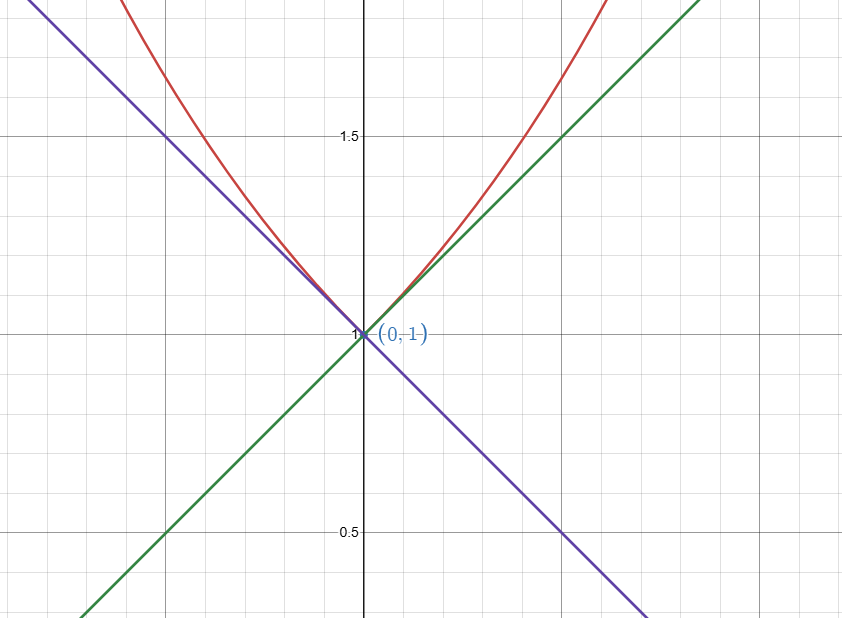
\includegraphics[width=0.7\textwidth]{pic/p5s2.png}
\end{figure}

可见其次微分为 \([-1,1]\).
\paragraph{解(c)}

平面\(P_1 : y = x_1 + x_2 - 1\) 和平面\(P_2 : x_1 - x_2 + 1\) 的交线为

\[ \begin{aligned}
    x_1 + x_2 - y & = 1 \\
    x_1 - x_2 - y & = -1
\end{aligned}\]

解得 \( x_1 = 1-2x_2, y = x-2x_2\) ,它的方向向量为 \(d= (-2,1,-1)\).

若次梯度为 \((a,b)\),那么其在空间中对应的平面的法向量为\( t = (\frac{1}{a},\frac{1}{b},1)\) 或\(t = (b,a,ab)\) , 有 \(t \bot d\),即 \(t \cdot d = 0\)

考虑过$(1,1,1)$ 且垂直于 $t$的平面$P_3: -2x_1 +x_2 - y = -2$, $P_1$和$P_2$ 与其交线分别为 
$l_1 : x_1 = 1,x_2 = y$ 和$l_2 : x_1 = 3-2y,x_2 = 4-3y$,   其方向向量分别为 $d_1 = (0,1,1)$, $d_2 = (-2,-3,1)$

以$(1,1,1)$为基点,$\{(1,2,0),(0,1,1)\}$为基向量建立坐标系,在该坐标系中$d_1 = (-2,1),d_2 = (0,1)$

\begin{figure}[H]
    \centering
    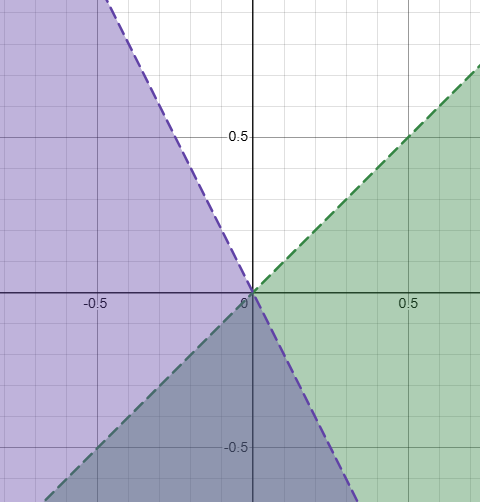
\includegraphics[width=0.7\textwidth]{pic/p5s3.png}
\end{figure}

在该坐标系中,一条直线过(0,0),并处于有色范围之中,该直线为 $y = kx \quad (-2 \leq k \leq 1)$, 该直线在原坐标系中的点以参数坐标格式为$(1+r,1+(2+k)r,1+kr)$,与向量$d$张成的平面,其上的点以参数坐标描述为 $(1+r - 2t,1+ (2+k)r +t, 1+kr-t)$,该平面上的点p 与$(1,1,1)$的差 $g = (r - 2t,(2+k)r + t , kr-t)$,每个都是合法的梯度向量

于是原函数的次微分为 \(\{(\frac{kr-t}{r-2t},\frac{kr-t}{(2+k)r-t}) | k \in [-2,1], r,t \in \mathbb{R}\}\)


\section{}

用 DFP 方法求解:

\[\min 10x_1^2 + x_2^2\]

取初始H矩阵为单位阵,即$H_0 = I, x_0 = (\frac{1}{10},1)^T$,做精确一维搜索。

\paragraph{解}

见:

输出为:
\begin{lstlisting}
one_d_min_try(test1, 0, 1) = (1.0, 4.0)
fibonacci_subsequence(test1, l, r, 0.03) = Solution(2.001271645021645, -0.9999983829189389)
davidon_flether_powell(test_f, test_g, x_0; eps = 0.03) = [-0.0003436853884885571, 0.005152432067100199]
\end{lstlisting}

\section{}

用 BFGS 法求解问题a

\[\min x_1^2 + 4x_2^2 - 4x_1 -8x_2\]

取初始H矩阵为单位阵,即$H_0 = I, x_0 = (0,0)^T$,做精确一维搜索。


见:

输出为:
\begin{lstlisting}
Converged after 145 iterations.
BFGS x_min = [1.9999996028522085, 0.9999999356472791], y=-7.999999999999826
\end{lstlisting}

\section{}

请用精确一维搜索来求解

\[\min x_1^2 + x_2^2 - x_1x_2 -10x_1 - 4x_2 + 60\]

取 $x_0 = (0,0)^T$

\begin{enumerate}[(a)]
    \item DFP 方法,$H_0 = I$;
    \item BFGS 方法,$H_0 = I$;
    \item FR 共轭梯度法,$\epsilon = 10^{-6}$, 初始点可设为 $x_0 = (0,0)^T$或其他解
\end{enumerate}

\section{}
请证明梯度下降法和牛顿法的收敛性,并采用梯度法来迭代求解二次规划问题的收敛
性分析。

\paragraph{证明}

\subsection{梯度下降法的收敛性}

梯度下降法的基本思想是沿着负梯度方向更新参数,以找到函数的局部最小值。假设我们有一个可微的目标函数 $f: \mathbb{R}^n \to \mathbb{R}$,其梯度为 $\nabla f(x)$,并且假设它是 Lipschitz 连续的,即存在常数 $L > 0$,使得:
\[
\|\nabla f(x) - \nabla f(y)\| \leq L \|x - y\| \quad \forall x, y \in \mathbb{R}^n
\]

\subsubsection{收敛性证明}

1. \textbf{更新规则}:
   \[
   x_{k+1} = x_k - \alpha_k \nabla f(x_k)
   \]
   其中 $\alpha_k$ 是步长。

2. \textbf{函数值下降}:
   利用泰勒展开:
   \[
   f(x_{k+1}) \leq f(x_k) + \nabla f(x_k)^T (x_{k+1} - x_k) + \frac{L}{2} \|x_{k+1} - x_k\|^2
   \]
   代入更新规则后,得到:
   \[
   f(x_{k+1}) \leq f(x_k) - \alpha_k \|\nabla f(x_k)\|^2 + \frac{L \alpha_k^2}{2} \|\nabla f(x_k)\|^2
   \]

3. \textbf{选择合适的步长}:
   选择 $\alpha_k$ 满足 $0 < \alpha_k < \frac{1}{L}$,则可以证明:
   \[
   f(x_{k+1}) < f(x_k)
   \]
   这表明梯度下降法在每一步都能减少目标函数的值。

4. \textbf{收敛性}:
   通过对函数值的递减性和有界性,可以得出梯度下降法在适当条件下是收敛的。

\subsection{牛顿法的收敛性}

牛顿法利用二阶导数信息来加速收敛,主要用于优化目标函数。

\subsubsection{收敛性证明}

1. \textbf{更新规则}:
   \[
   x_{k+1} = x_k - H^{-1} \nabla f(x_k)
   \]
   其中 $H$ 是目标函数的海森矩阵。

2. \textbf{局部收敛性}:
   若 $x^*$ 是 $f$ 的局部极小点,且 $H$ 在 $x^*$ 处是正定的,则牛顿法在 $x$ 足够接近 $x^*$ 时具有二次收敛性。

3. \textbf{函数值的下降}:
   通过泰勒展开和海森矩阵的性质,可以证明牛顿法的收敛速度比梯度下降法快。

\subsection{二次规划问题的收敛性分析}

考虑二次规划问题:
\[
\min \frac{1}{2} x^T Q x + c^T x
\]
其中 $Q$ 是正定矩阵。

1. \textbf{梯度和海森矩阵}:
   \[
   \nabla f(x) = Qx + c
   \]
   \[
   H = Q
   \]

2. \textbf{收敛性分析}:
   - \textbf{梯度下降法}:利用上述收敛性证明,对于二次目标函数,选择合适的步长 $\alpha_k$ 后,函数值会逐步减小,最终收敛至最优解。
   - \textbf{牛顿法}:因为 $Q$ 是正定的,牛顿法会在每一步快速收敛到最优解。

\subsection{结论}

梯度下降法和牛顿法在适当条件下都具有收敛性。对于二次规划问题,利用梯度法可以有效地达到最优解,且牛顿法通常收敛更快。通过选择合适的步长和利用二阶信息,可以加速收敛过程。

\section{}
总结无约束优化求解的基本思想,思考如何将非凸优化问题转化为凸优化问题,如何将
有约束问题转化为无约束问题。

\paragraph{答}

无约束优化问题的基本目标是寻找一个变量集合 $x \in \mathbb{R}^n$,使得目标函数 $f(x)$ 达到最小值。无约束优化的基本思想可以概述为以下几个步骤:

1. \textbf{目标函数的选择}:选择一个需要优化的目标函数 $f(x)$,该函数通常需要满足可微性条件,以便计算其梯度和海森矩阵。

2. \textbf{初始点的选择}:选择一个合适的初始点 $x_0$,为优化算法提供起始位置。

3. \textbf{迭代更新}:利用梯度信息或二阶导数信息,采用优化算法(如梯度下降法、牛顿法等)逐步更新解的值,直到满足收敛条件。

4. \textbf{收敛性检查}:根据设定的收敛标准(如梯度范数、函数值变化等)判断是否达到最优解,若未达到,则继续迭代。

\subsection{非凸优化问题转化为凸优化问题}

非凸优化问题的挑战在于目标函数或约束条件的非凸性。为了将非凸优化问题转化为凸优化问题,可以采用以下方法:

1. \textbf{局部凸化}:在非凸区域内通过局部线性化或二次近似来构建一个局部凸模型。这可以通过泰勒展开来实现,使得在当前点附近的优化问题变为凸问题。

2. \textbf{凸包方法}:使用凸包技术,通过引入辅助变量和约束条件,将非凸区域“包裹”在一个凸区域内,从而简化问题。

3. \textbf{松弛方法}:将非凸问题中的某些约束放宽,转而优化一个较为简单的凸问题。

\subsection{有约束优化问题转化为无约束问题}

将有约束优化问题转化为无约束问题的常用方法包括:

1. \textbf{拉格朗日乘子法}:通过引入拉格朗日乘子,将约束条件融入目标函数,构建拉格朗日函数 $L(x, \lambda) = f(x) + \lambda^T g(x)$,其中 $g(x)$ 为约束条件。优化拉格朗日函数可以在一定程度上处理约束问题。

2. \textbf{惩罚函数法}:在目标函数中添加惩罚项,使得违背约束的解会受到惩罚,从而引导优化过程朝向满足约束的解。形式为:
   \[
   \tilde{f}(x) = f(x) + \rho \cdot P(g(x))
   \]
   其中 $P(g(x))$ 是惩罚函数,$\rho$ 是惩罚系数。

3. \textbf{投影法}:在每一步迭代后,将解投影到约束集上,以确保解始终满足约束条件。这在处理简单约束时尤其有效。

通过上述方法,可以有效地将非凸优化问题转化为凸优化问题,以及将有约束问题转化为无约束问题,从而利用有效的优化算法进行求解。

\section{}

请将最速下降法、牛顿法、修正牛顿法的计算公式进行统一描述,并体会变尺度法的基
本思想。 

\paragraph{答}

在优化算法中,最速下降法、牛顿法和修正牛顿法是常用的迭代方法,它们的计算公式可以统一描述为以下形式:

\subsection{最速下降法}

最速下降法通过沿着负梯度方向进行更新,公式为:
\[
x_{k+1} = x_k - \alpha_k \nabla f(x_k)
\]
其中,$x_k$ 是第 $k$ 次迭代的点,$\nabla f(x_k)$ 是在该点的梯度,$\alpha_k$ 是步长。

\subsection{牛顿法}

牛顿法利用二阶导数信息进行更新,其迭代公式为:
\[
x_{k+1} = x_k - H^{-1} \nabla f(x_k)
\]
其中,$H$ 是目标函数的海森矩阵,$H^{-1}$ 是海森矩阵的逆矩阵。

\subsection{修正牛顿法}

修正牛顿法在每次迭代中更新一个近似的海森矩阵,更新公式为:
\[
x_{k+1} = x_k - B_k^{-1} \nabla f(x_k)
\]
其中,$B_k$ 是第 $k$ 次迭代的近似海森矩阵,通常通过BFGS或DFP等方法进行更新。

\subsection{变尺度法的基本思想}

变尺度法(Variable Metric Method)是一种优化方法,其基本思想是通过引入变量的尺度信息来改善搜索方向。与梯度下降法相比,变尺度法在更新过程中考虑了目标函数的几何形状,使得优化过程更加高效。

具体而言,变尺度法在每次迭代中使用一个变尺度矩阵 $B_k$ 来调整搜索方向,迭代公式为:
\[
x_{k+1} = x_k - \alpha_k B_k^{-1} \nabla f(x_k)
\]
通过对 $B_k$ 的选择,变尺度法能够在不同的方向上自适应调整步长,从而加快收敛速度,尤其是在处理长宽不同的目标函数时。

这种方法在处理高维和非线性优化问题时尤其有效,可以有效克服传统方法在收敛速度和稳定性方面的局限性。


\section{}

尝试采用深度学习中的随机梯度下降算法中各种一阶改进的优化算法来求解上述习题
中的典型问题。

\section{}

自己查看已有的深度学习模型,训练中其参数的变化是否服从低维特性?尝试画出这
些变化的分布。

\section{}

查阅一阶优化算法的最新加速算法思想,并总结其基本思路。(可查阅北大林宙辰老师
的英文版书籍)。

\section{}

请查阅资料给出Krylov子空间方法的基本思想,并讨论子空间投影的典型应用。尝试调
用GMRES求解典型的线性方程组,给出基本的结果。讨论GMRES方法和共轭梯度法的异同。

\section{}

请给出共轭函数的定义,理解如何求解共轭函数,并思考共轭函数和对偶性的联系。

\paragraph{答}

\subsection{共轭函数的定义}

设 $f: \mathbb{R}^n \to \mathbb{R}$ 是一个下半连续的凸函数,其共轭函数 $f^*: \mathbb{R}^n \to \mathbb{R}$ 定义为:
\[
f^*(y) = \sup_{x \in \mathbb{R}^n} \left( \langle y, x \rangle - f(x) \right)
\]
其中,$\langle y, x \rangle$ 表示 $y$ 和 $x$ 的内积。共轭函数 $f^*(y)$ 描述了原函数 $f(x)$ 的“对偶”性质。

\subsection{求解共轭函数}

求解共轭函数的步骤通常包括:

1. \textbf{计算内积}:对给定的 $y$,计算表达式 $ \langle y, x \rangle - f(x) $。

2. \textbf{取极大值}:通过求解上式的极大值来找到共轭函数。通常需要对 $x$ 进行求导并设置导数为零,解出 $x$ 的表达式。

3. \textbf{代入回原式}:将求得的 $x$ 的表达式代入到原式中,得到 $f^*(y)$ 的具体形式。

\subsection{共轭函数与对偶性的联系}

共轭函数与对偶性密切相关。在优化中,对偶性是指原问题的解与其对偶问题的解之间的关系。具体而言:

1. \textbf{对偶问题的构造}:通过原问题的 Lagrangian 函数,可以构造出对偶问题,其中对偶目标函数通常可以表示为原函数的共轭函数。

2. \textbf{强对偶性}:在某些条件下(如 Slater 条件),原问题的最优值与对偶问题的最优值相等。这种情况下,可以利用共轭函数来求解对偶问题。

3. \textbf{几何解释}:共轭函数在几何上反映了原函数的凸性特征,特别是在优化中,原函数和对偶函数之间的关系可以通过各自的切平面(subgradient)来理解。

因此,共轭函数不仅是优化理论中的基本工具,也是理解对偶性的重要桥梁。

\end{document}